\subsection{ResUnet architectures}
\label{sec:resunets}

Building on the architecture described in \cref{sec:unets}, multiple variants have been proposed, each exploiting more or less substantial tuning of some of its building blocks.
One of such derived versions is the so-called \textit{deep ResUnet} \cite{deep_resunet}, whose main difference is the adoption of \textit{residual units} \cite{residual_units} instead of unet blocks (see \cref{fig:residual_units}  for a visual comparison).
%Although the latter constitutes a whole family of architectures on its own -- and again, multiple versions are available with slight adaptations --, its main difference is the adoption of \textit{residual units} \cite{residual_units} instead of unet block.
% \Cref{fig:residual_units} reports a diagram of the above block
\begin{figure}
\centerline{
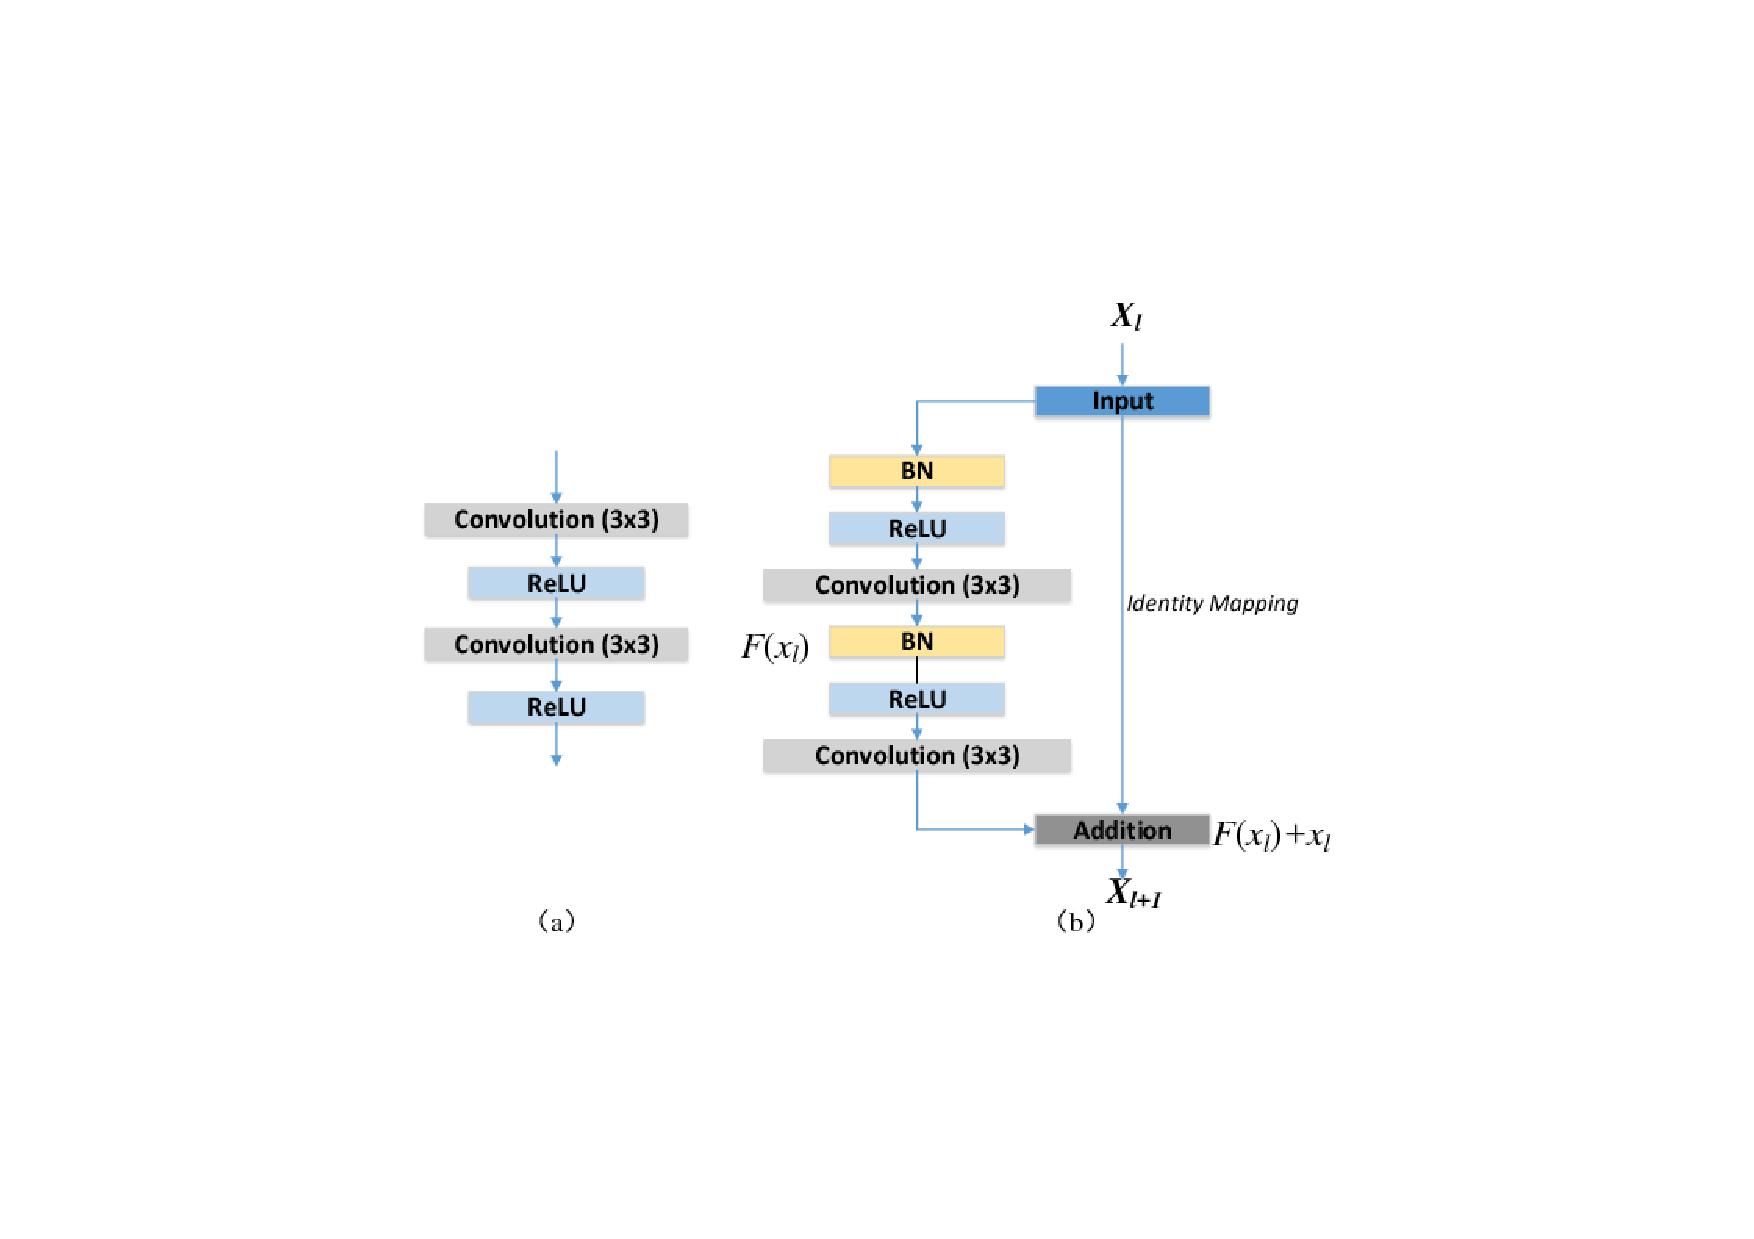
\includegraphics[width=\textwidth]{figures/130_methods/residual_unit.pdf}
}
\caption{\textbf{Unet versus Residual units.} Building blocks of neural networks. (a) Plain neural unit used in the Unet. (b) Residual unit with identity mapping used in the ResUnet model.
This figure is borrowed from \protect \citeA{deep_resunet}
% The shortcut-connections along the encoding-path are supported by a 1$\times$1 convolution to enable the final sum before the max-pooling operation.
} \label{fig:residual_units}
\end{figure}

The motivation behind the last modifications is to contrast the vanishing gradient \cite{vanishing_gradient} issue that generally affects the Unet models.
In practice, the deep architecture poses a severe challenge related to the backpropagation of the gradients during the learning phase.
In fact, each training iteration updates the network parameters by an amount proportional to the partial derivative of the loss function with respect to the previous weight values.
Specifically, the backpropagation algorithm is based on chained multiplications that propagate such gradients backward in the network to update all layers' parameters.
%to flow backward from the output layer to the initial ones.
However, this reverse flow may entail repeated multiplications of small values ($\leq1$) that cause the backpropagated gradients to ``vanish" -- i.e. to approach 0.
When that is the case, the update rule implies that network weights are also shrunk towards 0.
Consequently, the corresponding connections between neurons will be deactivated in the next forward pass, thus preventing the full exploitation of the available information and hampering the learning phase.
Of course, the deeper the architecture, the higher the chances of incurring this drawback.
In this regard, the residual units represent an ingenious gimmick to mitigate the impact of vanishing gradients.
The idea is to leverage an identity mapping (also referred to as short-connection) parallel to the usual convolutional block, which is added to the result of the convolutions. 
In this way, the input information is directly propagated to the next layers and considered should it be relevant for the subsequent processing.
Also, batch normalization layers are typically added to stabilize the range of the input values.
As a result, residual units typically guarantee comparable performance with fewer parameters, meanwhile enhancing the convergence speed.

\begin{figure}
\centerline{
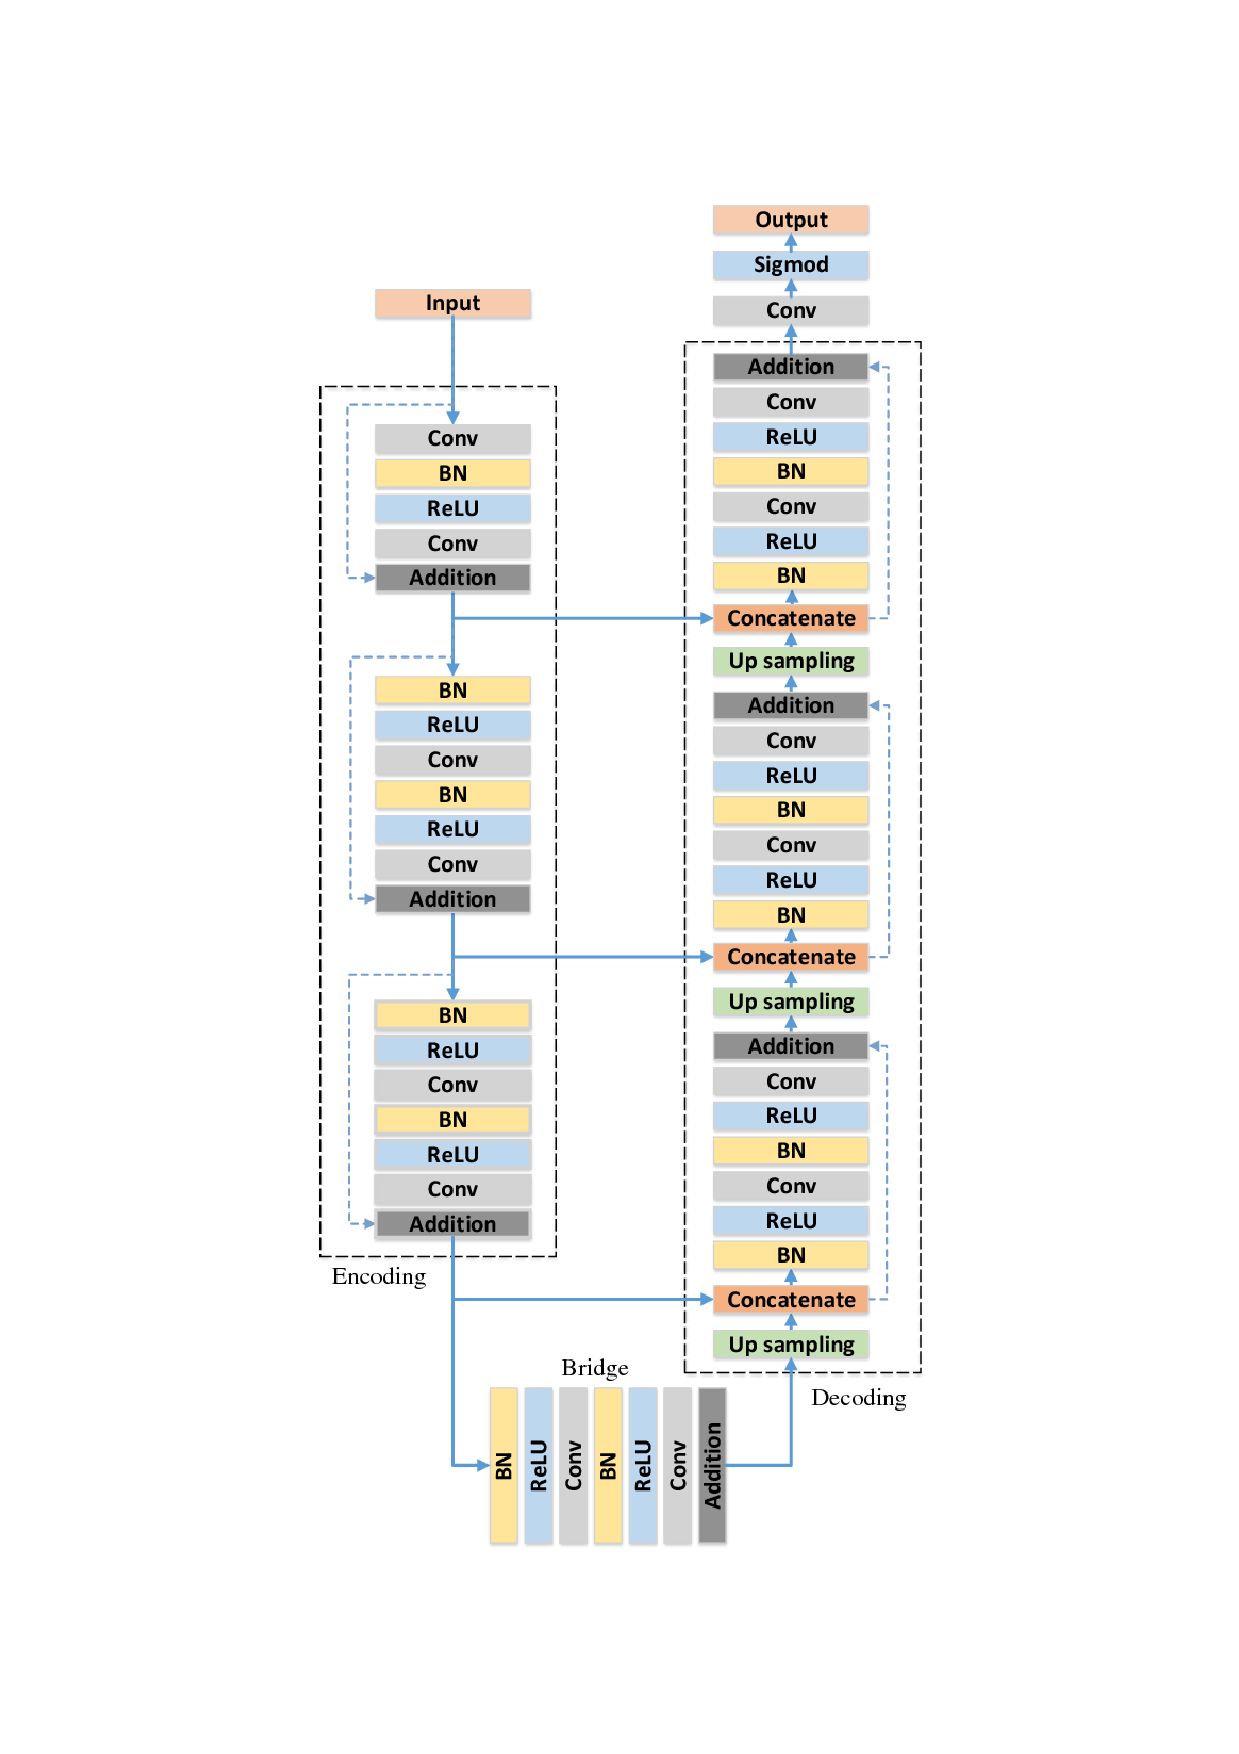
\includegraphics[width=0.9\textwidth]{figures/130_methods/resunet.pdf}
}
\caption{\textbf{Deep ResUnet architecture.}
This figure is borrowed from \protect \cite{deep_resunet}
} \label{fig:resunet_architecture}
\end{figure}
Given the advantages described above, we experiment with two architectures belonging to the ResUnet family inspired by the implementation presented in \citeA{deep_resunet} (see \cref{fig:resunet_architecture}).
In particular, a first version is obtained with the same components as in \cref{fig:resunet_architecture}, but using 16 initial filters -- instead of the 64 adopted in the original version \cite{deep_resunet} -- and scaling the following structure consequently.
Also, we adopt the exponential linear unit (Elu) \cite{clevert2015elu} rather than the ReLU activation.
The resulting model will be referred to as \textit{ResUnet} in the following.

Finally, we propose a slight modification to the above architecture specifically developed for our use case.
In particular, we add an initial 1$\times$1 convolution to simulate an RGB to grayscale conversion.
The advantage of doing so -- as opposed to applying a standard grayscale conversion -- is that the transformation is learned during training to improve the segmentation performance.
As a further modification, we insert an additional residual block having 5$\times$5 filters -- instead of 3$\times$3 -- at the end of the encoding path. 
This adjustment should provide the model with a larger field of view, thus fostering a better comprehension of the context surrounding the pixel to classify.
This kind of information can be beneficial, for example, when cells clump together and pixels on their boundaries have to be segmented. 
Likewise, the analysis of some background structures (\cref{fig:dataset:bright,fig:artifacts:stripe,fig:artifacts:macaroon}) can be improved by looking at a broader context.
The resulting architecture is reported in \cref{fig:cresunet_architecture} and it will be referred to as \textbf{cell ResUnet (c-ResUnet)} hereafter.

\newpage
\begin{figure}
\centerline{
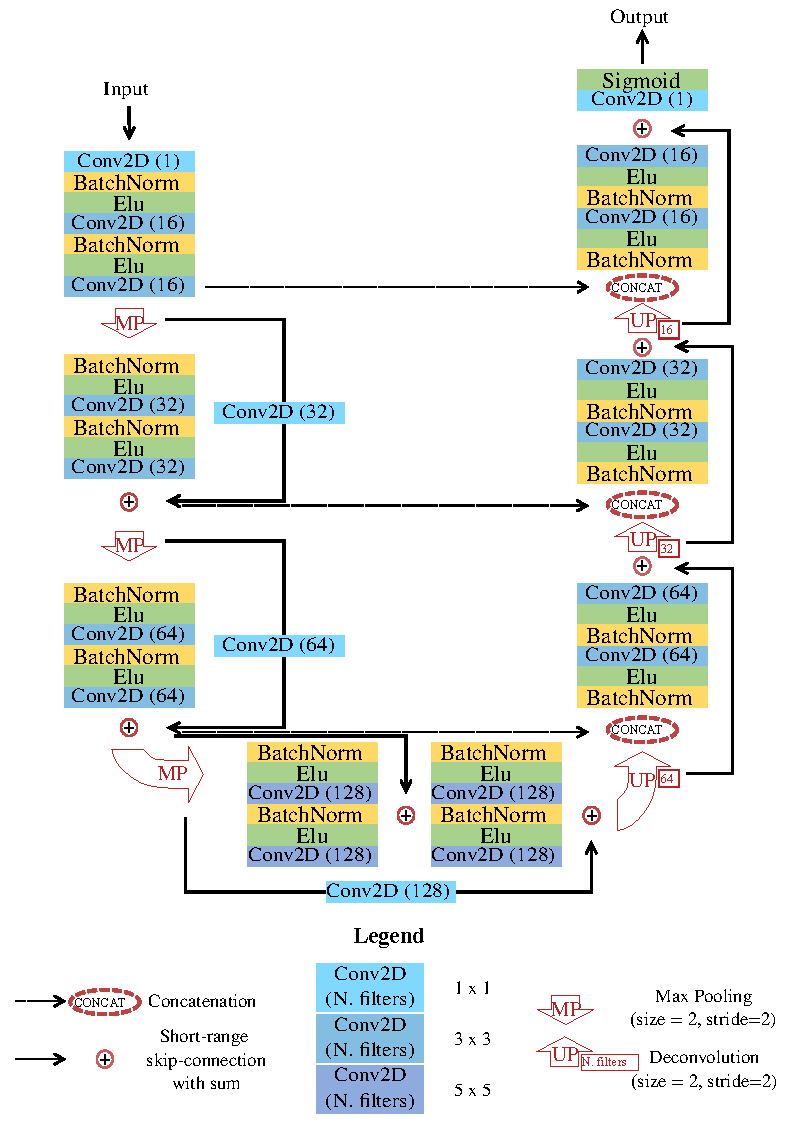
\includegraphics[width=0.8\textwidth]{figures/130_methods/c-resunet_architecture.pdf}
}
\caption{\textbf{c-ResUnet architecture.} Each box reports an element of the entire architecture (individual descriptions in the legend). 
% The shortcut-connections along the encoding-path are supported by a 1$\times$1 convolution to enable the final sum before the max-pooling operation.
} \label{fig:cresunet_architecture}
\end{figure}